\documentclass[10pt]{beamer}
\usepackage{hyperref}
\usepackage[T1]{fontenc}

% other packages
\usepackage{latexsym,amsmath,xcolor,multicol,booktabs,calligra}
\usepackage{graphicx,pstricks,listings,stackengine}

% packages and settings for bibtex 

\usepackage{animate}
%\defbibheading{reference}{\section*{参考文献}}   % heading for bibtex
\usepackage{ascmac}
\usepackage{fancybox}

\author[Shuta Nakajima]{Shuta Nakajima (Meiji University)}
\title{On the upper tail large deviation rate function for chemical distance}
%\subtitle{TAP approach to spin glass models}
\institute{ Joint work with Barbara Demin (CNRS)}
%\date{2023年12月18日}
\date{\today}
\usepackage{ucas}
\newtheorem{Def}{Definition}
\newtheorem{thm}{Theorem}
\newtheorem*{thm*}{Theorem}
\newtheorem{ass}{Assumption}
\newtheorem{lem}{Lemma}
\newtheorem*{lem*}{Lemma}
\newtheorem{prop}[thm]{Proposition}
\newtheorem{cor}{Corollary}
\newtheorem*{remark}{Remark}
\newtheorem{assumption}{Assumptions}

\newcommand{\N}{\mathbb{N}}
\newcommand{\R}{\mathbb{R}}

\renewcommand{\P}{\mathbb{P
}}
\newcommand{\E}{\mathbb{E}}
\newcommand{\Z}{\mathbb{Z}}
\renewcommand{\L}{\mathbb{L}}

\newcommand{\cev}[1]{\accentset{\leftarrow}{#1}}
\newcommand{\e}{\epsilon}
\newcommand{\kG}{\mathcal{G}}
\newcommand{\kD}{\mathcal{D}}
\newcommand{\kC}{\mathcal{C}}

\newcommand{\kA}{\mathcal{A}}
\renewcommand{\d}{\mathsf{d}}
\newcommand{\ds}{\displaystyle}
\newcommand{\ts}{\textstyle}
\newcommand{\bra}{\langle}
\newcommand{\ket}{\rangle}
\newcommand{\supp}{\mathrm{supp}}
\newcommand{\ssup}[1]{{\scriptscriptstyle{({#1}})}}
\newcommand{\DL}{\Delta^{\hspace{-1pt}\ssup\epsilon}}
\newcommand{\DG}{\nabla^{\ssup\epsilon}}
\newcommand{\pev}{\lambda_{D_{\epsilon}psilon, \xi}}
\newcommand{\pef}{g_{D_{\epsilon}psilon, \xi}}
\newcommand{\F}{\mathcal{F}}
% defs
\def\cmd#1{\texttt{\color{red}\footnotesize $\backslash$#1}}
\def\env#1{\texttt{\color{blue}\footnotesize #1}}
\definecolor{deepblue}{rgb}{0,0,0.5}
\definecolor{deepred}{rgb}{0.6,0,0}
\definecolor{deepgreen}{rgb}{0,0.5,0}
\definecolor{halfgray}{gray}{0.55}

\def\be#1{\begin{equation*}#1\end{equation*}}
\def\ben#1{\begin{equation}#1\end{equation}}
\def\bea#1{\begin{eqnarray*}#1\end{eqnarray*}}
\def\bean#1{\begin{eqnarray}#1\end{eqnarray}}
\def\al#1{\begin{align*}#1\end{align*}}
\def\aln#1{\begin{align}#1\end{align}}
\lstset{
    basicstyle=\ttfamily\small,
    keywordstyle=\bfseries\color{deepblue},
    emphstyle=\ttfamily\color{deepred},    % Custom highlighting style
    stringstyle=\color{deepgreen},
    numbers=left,
    numberstyle=\small\color{halfgray},
    rulesepcolor=\color{red!20!green!20!blue!20},
    frame=shadowbox,
}


\begin{document}

\begin{frame}
    \titlepage
\end{frame}

\section{Introduction and models}

\begin{frame}{Percolation model}
    \begin{itemize}
    \item Let $\E^d=\{\{x,y\}|~x,y\in \Z^d;\,|x-y|_1=1\}$.
    \item $(\tau_e)_{e\in \E^d}$: i.i.d. RVs on $\{1,\infty\}$ such that  $$\P(\underbrace{\tau_e=1}_{{\color{red}open}})=1-\P(\underbrace{\tau_e=\infty}_{{\color{blue}closed}})\equiv p\in [0,1].$$
  %  \item We write $x\leftrightarrow y$ if $\exists \gamma:x\to y$ in $\kG_p$.
       \item Let $\mathcal{G}_p=(\Z^d,\{e\in \E^d|~\tau_e=1\})$ ({\color{red}{percolation graph}}).
    \end{itemize}
    ~\\
  \vspace{16mm}
\end{frame}
\begin{frame}{Percolation model}
    \begin{itemize}
    \item Let $\E^d=\{\{x,y\}|~x,y\in \Z^d;\,|x-y|_1=1\}$.
    \item $(\tau_e)_{e\in \E^d}$: i.i.d. RVs on $\{1,\infty\}$; $\P(\tau_e=1)=1-\P(\tau_e=\infty)\equiv p.$
  %  \item We write $x\leftrightarrow y$ if $\exists \gamma:x\to y$ in $\kG_p$.
       \item Let $\mathcal{G}_p=(\Z^d,\{e\in \E^d|~\tau_e=1\})$ ({\color{red}{percolation graph}}).
    \end{itemize}
     \begin{figure}[htpb]
        \begin{center}
          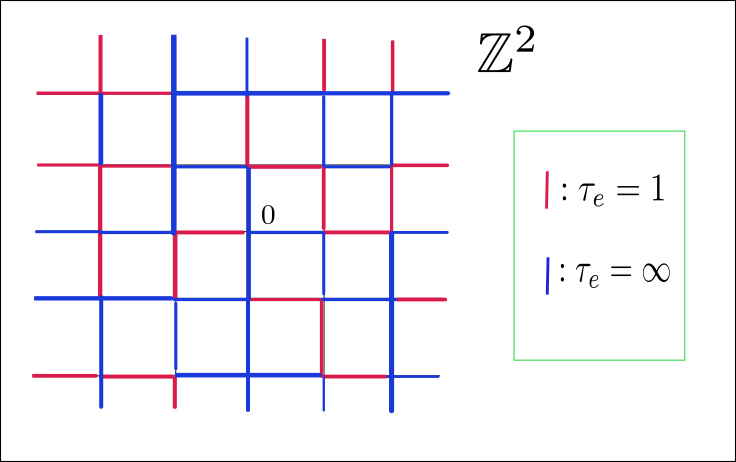
\includegraphics[width=0.6\linewidth]{percolation.png}
        \end{center}
        \caption{A typical percolation graph}
    \end{figure}
\end{frame}

\begin{frame}{Percolation model}
    \begin{itemize}
    \item Let $\E^d=\{\{x,y\}|~x,y\in \Z^d;\,|x-y|_1=1\}$.
    \item $(\tau_e)_{e\in \E^d}$: i.i.d. RVs on $\{1,\infty\}$; $\P(\tau_e=1)=1-\P(\tau_e=\infty)\equiv p.$
       \item Let $\mathcal{G}_p=(\Z^d,\{e\in \E^d|~\tau_e=1\})$ ({\color{red}{percolation graph}}).
    \end{itemize}
     \begin{figure}[htpb]
        \begin{center}
          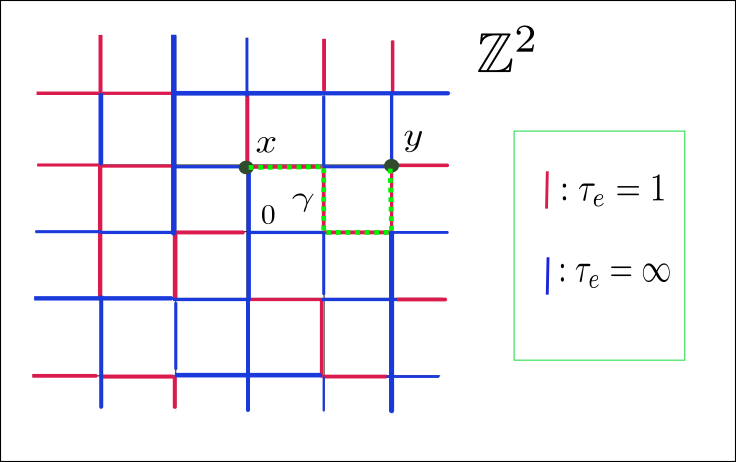
\includegraphics[width=0.6\linewidth]{path.png}
        \end{center}
        \caption{A typical percolation graph and an open path}
    \end{figure}
\end{frame}
\begin{frame}{Percolation model}
    \begin{itemize}
    \item Let $\E^d=\{\{x,y\}|~x,y\in \Z^d;\,|x-y|_1=1\}$.
   \item $(\tau_e)_{e\in \E^d}$: i.i.d. RVs on $\{1,\infty\}$ such that  $$\P(\tau_e=1)=1-\P(\tau_e=\infty)\equiv p\in [0,1].$$
  \item Let $\mathcal{G}_p=(\Z^d,\{e\in \E^d|~\tau_e=1\})$ ({\color{red}{percolation graph}}).
  \item We write $x\leftrightarrow y$ if $\exists \gamma:x\to y$ in $\kG_p$.
  \item We define the cluster containing $x\in \Z^d$: 
  $$\mathcal{C}(x)\equiv \{y\in \Z^d|~x\leftrightarrow y\},\quad x\in \Z^d.$$
    \end{itemize}
\end{frame}

\begin{frame}{Chemical distance}
    \begin{itemize}
           \item $(\tau_e)_{e\in \E^d}$: i.i.d. RVs on $\{1,\infty\}$ such that  $$\P(\tau_e=1)=1-\P(\tau_e=\infty)\equiv p\in [0,1].$$
  \item Let $\mathcal{G}_p=(\Z^d,\{e\in \E^d|~\tau_e=1\})$ ({\color{red}{percolation graph}}).
  \item We write $x\leftrightarrow y$ if $\exists \gamma:x\to y$ in $\kG_p$.
  \item We define the cluster containing $x\in \Z^d$: 
  $$\mathcal{C}(x)\equiv \{y\in \Z^d|~x\leftrightarrow y\},\quad x\in \Z^d.$$
            \item Let $\mathcal{D}(x,y)$ be the graph distance on $\mathcal{G}_p$ ({\color{red} chemical distance}):       \al{
            \mathcal{D}(x,y)&\equiv \inf\{|\gamma|:~\gamma:x\to y\text{ in }\mathcal{G}_p\}.
         %   &=\inf\left\{\sum_{e\in \gamma}\tau_e:~\gamma:x\to y\right\}.
            }
    \end{itemize}
\end{frame}

\section{History and Previous research}
\begin{frame}{Percolation theory and phase transition}
\begin{itemize}
    \item Percolation model was introduced by Broadbend and Hammersley in 1957 to model a fluid flow in porous media.
%    \item There have been many studies on the geometry in $\kG_p$, in particular, the clusters $\kC(x)$ ($x\in \Z^d$).
\end{itemize}

\begin{thm}[Aizenmann-Kesten-Newman '85]
Suppose $d\geq 2$. There exists $p_c(d)\in (0,1)$ such that
\begin{itemize}
    \item for $p<p_c(d)$ ({\color{red}{subcritical regime}}),
$$
  \P(|\kC(x)|<\infty,\quad\forall x\in \Z^d)=1;$$
   \item for $p>p_c(d)$ ({\color{red}{supercritical regime}}),
  $$\P(\exists x;\,|\kC(x)|=\infty;\quad\forall y\notin\kC(x), \,|\kC(y)|<\infty)=1.
$$
\end{itemize}
\end{thm}
When $p>p_c(d)$, we denote by $\mathcal{C}_\infty$ the (unique) infinite cluster.
\end{frame}

\begin{frame}{History of chemical distance}
  \begin{itemize}
    \item The name ``chemical distance'' was suggested by Sage Alexander around 1985.
    \item The physicists have been interested in the growth exponent $\alpha(d)$ at $p=p_c(d)$:
      $$\kD(0,n\mathbf{e}_1)\asymp n^{\alpha(d)}.$$
    \item No consensus on the value of $\alpha(d)$ even for $d=2$. 
    \item So far, almost all results between {\color{red}Chemical distance in supercritical percolation} and {\color{blue}Eden growth model (FPP with Exp)} have matched.\\

      \vspace{2mm}
      $\Rightarrow$ {\color{red}Chemical distance} belongs to KPZ universality class?
    \end{itemize}
  \end{frame}
\begin{frame}{Law of large numbers}
 \underline{\bf Notation}\\
    \vspace{2mm}
    $\kD(x)\equiv \kD(0,\lfloor x\rfloor).$\\
\begin{thm}[Garet-Marchand '04]
  For any $x\in \R^d$, there exists $\mu(x)\geq 0$ ({\color{red}time constant}); for any $\delta>0$,
$$\P(|\kD(nx)-n\mu(x)|>\delta n;\,0\leftrightarrow \lfloor nx\rfloor)\to 0.$$
\end{thm}
~\\
The theorem roughly says that $\kD(nx)\approx n\mu(x)$ whenever $0$ and $nx$ are connected in $\kG_p.$\\
\vspace{5mm}
\fbox{Next problems}
\begin{itemize}
\item Fluctuations
  \item Large deviations ({\color{red}Main theme in this talk!})
  \end{itemize}
\end{frame}

\begin{frame}{What is large deviations?}
    \begin{itembox}[t]{Large deviations?}
    Large deviations concern rare events and its probabilities.
    \end{itembox}
    ~\\
    \vspace{4mm}
We consider the following two events: given $\xi>0$ and $x\in \mathbb R^d$,
    \begin{align*}
& \{\kD(nx)<(1-\xi)\mu(x)n)\} \text{ ({\color{red}lower tail LD})},\\
   &    \{(1+\xi)\mu(x)n\leq \kD(nx)<\infty)\} \text{ ({\color{red} upper tail LD})}.
      \end{align*}
\end{frame}

\begin{frame}{Large deviations for the chemical distance}
    Suppose $d\geq 2$ and $p>p_c(d)$.
    \begin{thm}[Antal-Pisztora '96,\,Garet-Marchand '07]
    For any $x\in \R^d$ and $\epsilon>0$, there exists $c>0$ such that
    $$\P\left((1+\epsilon)\mu(x)n\leq \kD(nx)< \infty)\right)\leq e^{-c n}.$$
    \end{thm}
    \pause
    \begin{thm}[Garet-Marchand '07]
    For any $x\in \R^d$, the following limit exists and is negative or $-\infty$:
    $$\lim_{n\to\infty}\frac{1}{n}\log{\P\left(\kD(nx)< (1-\epsilon)\mu(x)n\right)}.$$
    \end{thm}
    The limit is called the {\color{red} rate function}. Our aim is to prove the existence of the rate function for upper LDP.
\end{frame}
\section{Main result}

\begin{frame}{Space-time cutpoint}
\vspace{-1mm}
\underline{\bf Notation} 
\begin{itemize}
    \item $\Lambda_N(x)\equiv x+[-N,N]^d$.
    \item $B_s(x)\equiv \{y\in \Z^d|~\kD(x,y)\leq s\}$,\quad$B_s\equiv B_s(0)$.
\end{itemize}
\vspace{-1mm}
\begin{Def}[Space-time cutpoint]
Fix $\alpha_d:=1-\frac{1}{6d}$. Given $s>0$ and $x\in \R^d$,
$$\mathcal{A}_{s,x}(n)\equiv\{\exists t\geq s n,\,\exists w\in \Lambda_{n^\alpha}(nx);\,\{w\}=B_t\setminus B_{t-1
}\}.$$
\end{Def}
\pause
     \begin{figure}[h]
        \begin{center}
            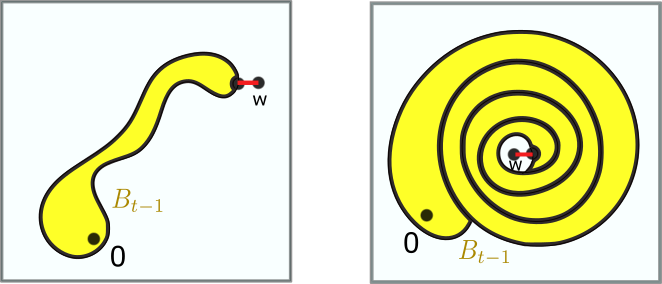
\includegraphics[width=0.7\linewidth]{examples.png}
        \end{center}
         \caption{Pedagogical example \quad v.s. \quad Pathological example}
    \end{figure}
\end{frame}
\begin{frame}{What is a cutpoint?}
  
     \begin{figure}[h]
        \begin{center}
            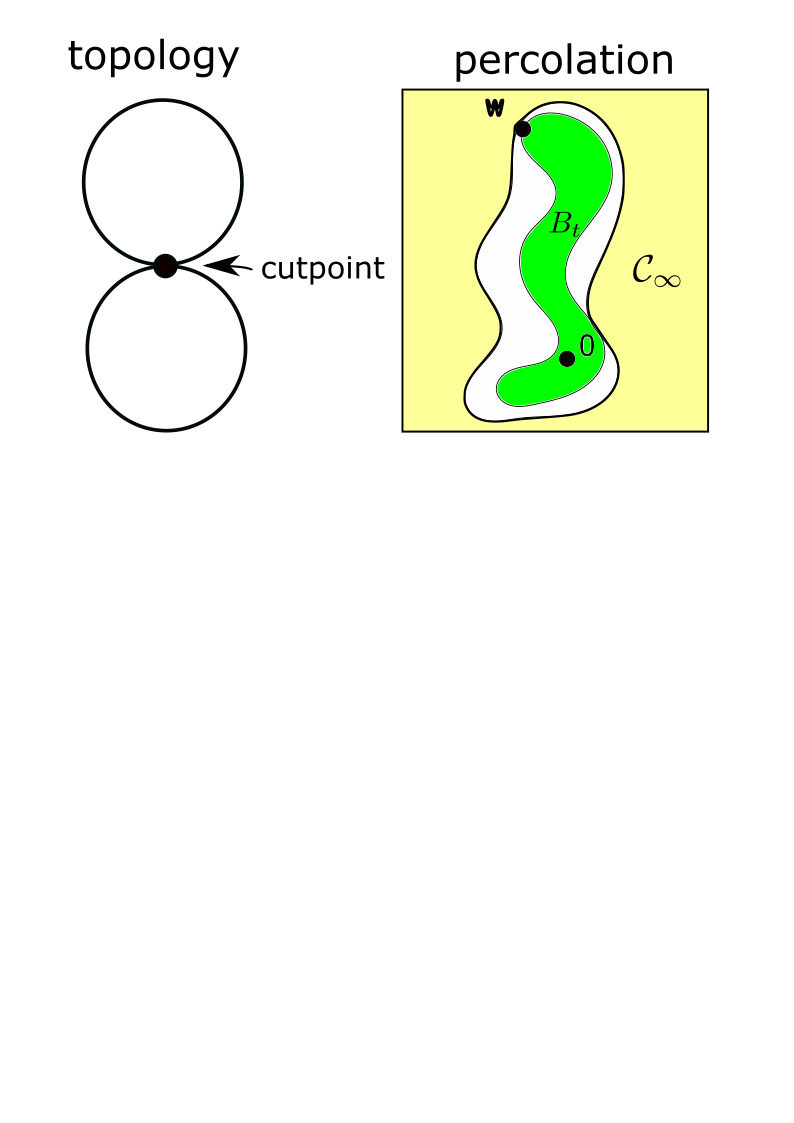
\includegraphics[width=1.1\linewidth]{topology.png}
        \end{center}
    \end{figure}
\end{frame}

\begin{frame}{Rate function for a space-time cutpoint}
  From now on, {\bf we always assume $d\geq 3$ and $p>p_c(d)$.}
\begin{thm}[Dembin-N 22+]
For any $s>0$ and $x\in \R^d$,
$$I(s,x):=\exists \lim_{n\to\infty}\frac{-1}{n}\log{\P\left(\mathcal{A}_{s,x}(n)\right)}>0.$$
Moreover, $I$ is convex and homogeneous, i.e.,
\al{
&I( \lambda s+(1-\lambda)s',\lambda x+(1-\lambda)x')\leq \lambda I( s,x)+(1-\lambda)I(s',x'),\\
&I(\lambda s,\lambda x)=\lambda I(s,x).
}
\end{thm}   
~\\
This $I$ is called the {\color{red} rate function} for a space-time cutpoint.
\end{frame}
\begin{frame}{Upper LDP rate function for chemical distance}
Given $\xi>0$ and $x\in \R^d$, we define
$$J(\xi,x)\equiv \inf\{I(s,u)|~s>0,u\in \R^d;\,s+\mu(x-u)>(1+\xi)\mu(x)\}.$$
\begin{thm}
  \begin{itemize}
  \item $J$ is continuous in $(\xi,x)$.
    \item For any $x\in \R^d$ and for any $\xi>0$ small enough,
      $$\lim_{n\to\infty}\frac{-1}{n}\log{\P\left((1+\xi)\mu(x)n\leq \kD(nx)< \infty)\right)}=J(\xi,x).$$
      \end{itemize}
\end{thm}    
\end{frame}
\section{Proof}
\begin{frame}{Proof}
For simplicity, we only consider $x=\mathbf{e}_1$. Then 
$$J(\xi)= \inf\{I(s,u)|~s>0,u\in \R^d;\,s+\mu(\mathbf{e}_1-u)>(1+\xi)\mu(\mathbf{e}_1))\}.$$
Our aim is to give a heuristic behind the proof of
$$\P\left((1+\xi)\mu(\mathbf{e}_1)n\leq \kD(n\mathbf{e}_1)< \infty)\right)\approx e^{-n J(\xi)}.$$
The core of the proof is
$$\text{Space-time cutpoint}\Leftrightarrow \{(1+\xi)\mu(\mathbf{e}_1)n\leq \kD(n\mathbf{e}_1)< \infty\}.$$
\end{frame}
\begin{frame}{Cutpoint$\Rightarrow$ Upper LDP}
Let $(s,u)$ such that
$$J(\xi)=I(s,u)\,\&\,s+\mu(\mathbf{e}_1-u)\geq (1+\xi)\mu(\mathbf{e}_1).$$
Suppose $\mathcal{A}_{s,u}(n)$.\\
\vspace{-8mm}
     \begin{figure}[h]
        \begin{center}
            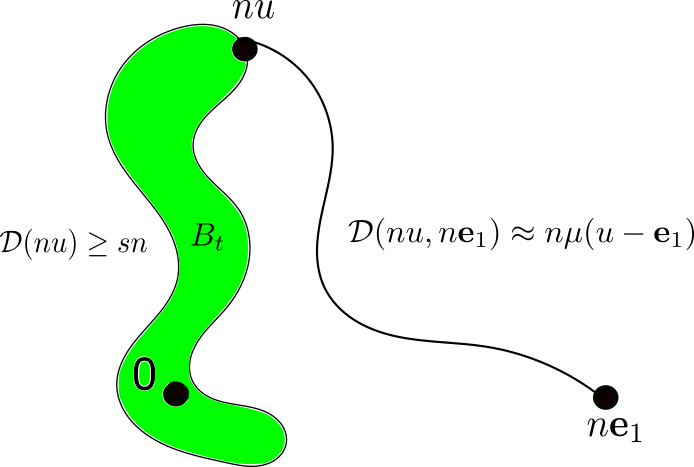
\includegraphics[width=0.6\linewidth]{LB.png}
        \end{center}
    \end{figure}
$$\infty>\kD(n\mathbf{e}_1)\geq sn+\mu(\mathbf{e}_1-u)n-o(n)\geq (1+\xi)\mu(\mathbf{e}_1)n-o(n).$$
$$\Rightarrow\hspace{2mm} \P(\kD(n\mathbf{e}_1)\in [ (1+\xi)\mu(\mathbf{e}_1)n,\infty))\geq \P(\mathcal{A}_{s,u}(n))\geq e^{-nI(s,u)}=e^{-nJ(\xi)}.$$
\end{frame}
\begin{frame}{Upper LDP $\Rightarrow $ Cutpoint I}
 Suppose $\kD(n\mathbf{e}_1)\in [ (1+\xi)\mu(\mathbf{e}_1)n,\infty)). $   Let 
    \al{
    s_n&\equiv\inf\{k\in \N|~|B_k(0)|\geq n^{7/4}\},\\
    t_n&\equiv \inf\{k\in \N|~|B_k(n\mathbf{e}_1)|\geq n^{7/4}\}.
    }
        \begin{figure}[h]
        \begin{center}
            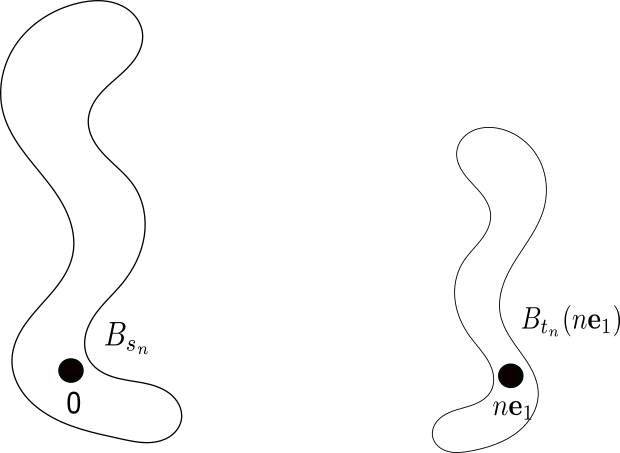
\includegraphics[width=0.6\linewidth]{Upper.png}
        \end{center}
    \end{figure}
\end{frame}

\begin{frame}{Upper LDP $\Rightarrow $ Cutpoint I}
 Suppose $\kD(n\mathbf{e}_1)\in [ (1+\xi)\mu(\mathbf{e}_1)n,\infty)). $   Let 
    \al{
    s_n&\equiv\inf\{k\in \N|~|B_k(0)|\geq n^{7/4}\},\\
    t_n&\equiv \inf\{k\in \N|~|B_k(n\mathbf{e}_1)|\geq n^{7/4}\}.
    }
        \begin{figure}[h]
        \begin{center}
            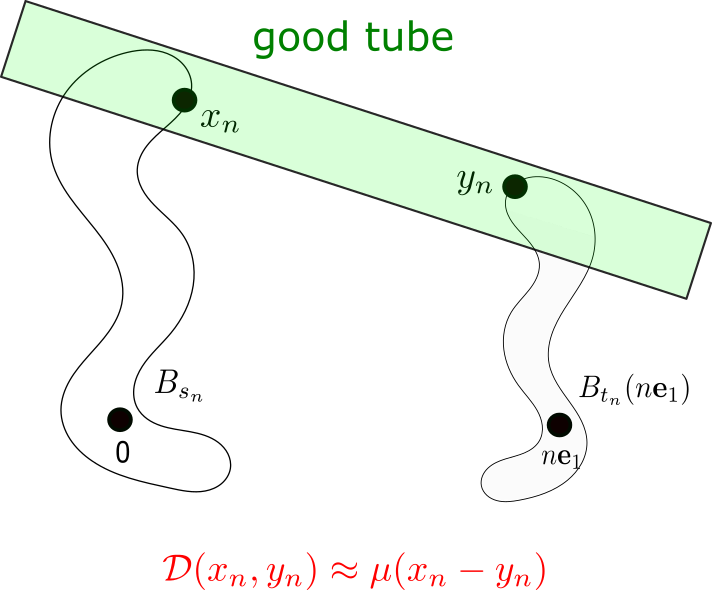
\includegraphics[width=0.6\linewidth]{gtube.png}
        \end{center}
    \end{figure}
\end{frame}
\begin{frame}{Upper LDP $\Rightarrow $ Cutpoint I}
 Suppose $\kD(n\mathbf{e}_1)\in [ (1+\xi)\mu(\mathbf{e}_1)n,\infty)). $   Let 
    \al{
    s_n&\equiv\inf\{k\in \N|~|B_k(0)|\geq n^{7/4}\},\\
    t_n&\equiv \inf\{k\in \N|~|B_k(n\mathbf{e}_1)|\geq n^{7/4}\}.
    }
    We find $x_n\in B_{s_n}(0)$ and $y_n\in B_{t_n}(n\mathbf{e}_1)$ such that
    $$\kD(x_n,y_n)\approx \mu(x_n-y_n).$$
   With $\overline{s}_n\equiv \kD(0,x_n)/n,\,\overline{t}_n\equiv \kD(y_n,n\mathbf{e}_1)/n,\,\overline{x}_n\equiv x_n/n,\,\overline{y}_n\equiv y_n/n$, 
\al{
  (1+\xi)\mu(\mathbf{e}_1)n&\leq \kD(0,n\mathbf{e}_1)\\
  &\leq \kD(0,x_n)+\kD(x_n,y_n)+\kD(y_n,n\mathbf{e}_1)\\
&\lesssim n \overline{s}_n+n\mu(\overline{x}_n-\overline{y}_n)+n \overline{t}_n.
}
$$\therefore\quad \mu(\overline{x}_n-\overline{y}_n)+\overline{s}_n+ \overline{t}_n\geq (1+\xi)\mu(\mathbf{e}_1).\qquad\qquad$$
\end{frame}

\begin{frame}{Upper LDP $\Rightarrow $ Cutpoint II}
    ``Making cutpoint'' lemma  realizes $$\kA_{\overline{s}_n,\overline{x}_n}(n)\cap (n\mathbf{e}_1+\kA_{\overline{t}_n,\overline{y}_n-\mathbf{e}_1}(n)).$$
  ~\\
     \begin{figure}[h]
        \begin{center}
            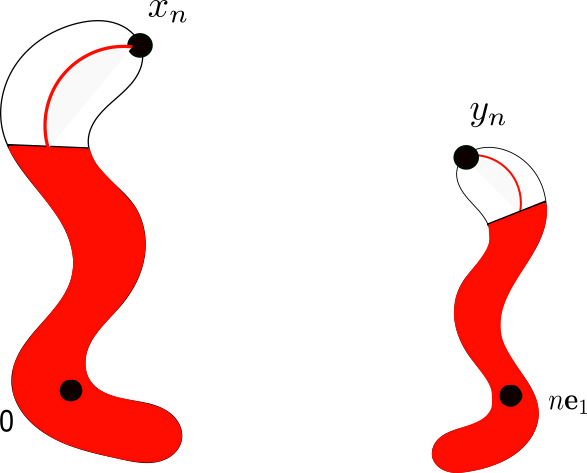
\includegraphics[width=0.7\linewidth]{UB.png}~\hspace{10mm}
        \end{center}
    \end{figure}
\end{frame}
\begin{frame}{Upper LDP $\Rightarrow $ Cutpoint III}
    Therefore, if $\xi$ is small enough, then
\al{
&\P(\kD(n\mathbf{e}_1)\in [(1+\xi)n\mu(\mathbf{e}_1),\infty))\\
&\leq \underset{\mu(x-y)+s+t\geq (1+\xi)\mu(\mathbf{e}_1)}{\sum_{x,y\in \Z^d/n,\,s,t\in \N/n}}\P(\kA_{s,x}(n)\cap (n\mathbf{e}_1+\kA_{t,y-\mathbf{e}_1}(n)))\\
&\approx  \sup_{\mu(x-y)+s+t\geq (1+\xi)\mu(\mathbf{e}_1)}\P(\kA_{s,x}(n)\cap (n\mathbf{e}_1+\kA_{t,y-\mathbf{e}_1}(n))) \\
&\approx \sup_{\mu(x-y)+s+t\geq (1+\xi)\mu(\mathbf{e}_1)}\P(\kA_{s,x}(n))\P (n\mathbf{e}_1+\kA_{t,y-\mathbf{e}_1}(n))\\
&\approx \exp{\left(n\sup_{\mu(x-y)+s+t\geq (1+\xi)\mu(\mathbf{e}_1)} -I(s,x)-I(t,y-\mathbf{e}_1)\right)}\\
&\leq \exp\left(-n\inf_{\mu(x-\mathbf{e}_1)+s\geq (1+\xi)\mu(\mathbf{e}_1)} I(s,x)))\right)=e^{-nJ(\xi)}. 
}
\end{frame}

\begin{frame}
Let $L_i^K(w)=\{w+k \mathbf{e}_i:~k\in \{-K,\cdots,K-1,K\}\}.$
\begin{lem}[Free line lemma]
There exists $i\in\{1,\cdots,d\}$ such that
    $$\P(\kA_{s,x}(n))\leq e^{o(n)}\P\left(
    \begin{array}{c}
    \exists t\geq s n,\,\exists w\in \Lambda_{n^\alpha}(nx);\\
    B_t\setminus B_{t-1}=\{w\}
,\quad
L_i^{n^\alpha}(w)\cap B_t=\{w\}
\end{array}
    \right).$$
\end{lem}
~\\
     \begin{figure}[h]
        \begin{center}
          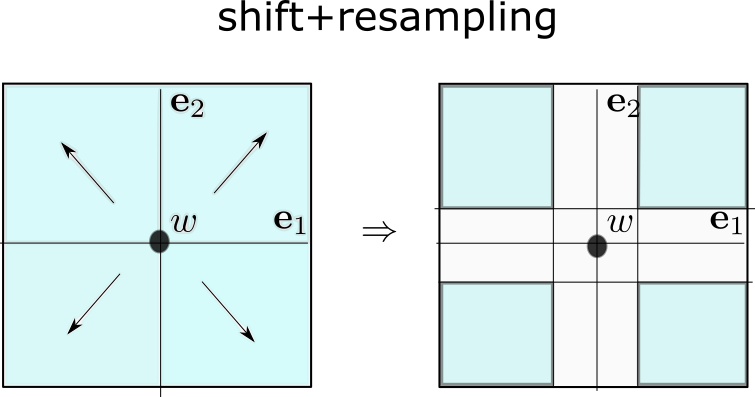
\includegraphics[width=0.7\linewidth]{shift.png}
        \end{center}
    \end{figure}
\end{frame}
\begin{frame}{Future works}
We list some open problems:\\

\begin{itemize}
    \item Upper LDP for large $\xi$.
%    \item 2D upper LDP for chemical distance ({\color{red}ongoing}).
    \item $\P(|B_{sn}|=O(n)|~\mathcal{A}_{s,x}(n))\to 1$.
    \item Rate function for multiple (space-time) cutpoints.
        \item Upper LDP for other percolation models.
\end{itemize}
    
\end{frame}
\end{document}